\documentclass[11pt,a4paper,fontset=fandol]{ctexart}

\usepackage{amsmath,amssymb,bm}
\usepackage{geometry}
\usepackage{enumitem}
\usepackage{fancyhdr}
\usepackage{lastpage}
\usepackage{xcolor}
\usepackage[most]{tcolorbox}
\usepackage{titlesec}
\usepackage{graphicx}
\usepackage{booktabs}
\usepackage{array}

\geometry{left=2.15cm,right=2.15cm,top=2.0cm,bottom=2.0cm}
\setlength{\parindent}{2em}
\setlength{\parskip}{0.22em}
\linespread{1.10}

\definecolor{mainblue}{RGB}{39,91,150}
\definecolor{lightblue}{RGB}{232,241,252}
\definecolor{darkgray}{RGB}{65,65,65}
\definecolor{lightgray}{RGB}{245,246,248}
\definecolor{warn}{RGB}{156,87,34}
\definecolor{softgreen}{RGB}{236,246,238}
\definecolor{deepgreen}{RGB}{63,123,74}

\titleformat{\section}{\large\bfseries\color{mainblue}}{}{0em}{}[\titlerule]
\titleformat{\subsection}{\normalsize\bfseries\color{darkgray}}{}{0em}{}
\titlespacing*{\section}{0pt}{0.85em}{0.42em}
\titlespacing*{\subsection}{0pt}{0.62em}{0.22em}

\setlist[enumerate]{leftmargin=2.2em,itemsep=0.22em,topsep=0.22em}
\setlist[itemize]{leftmargin=2.0em,itemsep=0.18em,topsep=0.18em}

\pagestyle{fancy}
\fancyhf{}
\lhead{\small 格物助航｜每日一练}
\rhead{\small 2026.6.9}
\cfoot{\small 第 \thepage\ 页 / 共 \pageref{LastPage} 页}
\renewcommand{\headrulewidth}{0.4pt}

\newtcolorbox{problemBox}{
 colback=lightblue,
 colframe=mainblue,
 arc=2mm,
 boxrule=0.7pt,
 left=1.0em,
 right=1.0em,
 top=0.75em,
 bottom=0.75em,
 before skip=0.55em,
 after skip=0.75em
}

\newtcolorbox{tipBox}{
 colback=lightgray,
 colframe=darkgray,
 arc=1.5mm,
 boxrule=0.5pt,
 left=0.9em,
 right=0.9em,
 top=0.55em,
 bottom=0.55em,
 before skip=0.45em,
 after skip=0.45em
}

\newtcolorbox{warnBox}{
 colback=white,
 colframe=warn,
 arc=1.5mm,
 boxrule=0.6pt,
 left=0.9em,
 right=0.9em,
 top=0.55em,
 bottom=0.55em,
 before skip=0.45em,
 after skip=0.45em
}

\newtcolorbox{ideaBox}{
 colback=softgreen,
 colframe=deepgreen,
 arc=1.5mm,
 boxrule=0.6pt,
 left=0.9em,
 right=0.9em,
 top=0.55em,
 bottom=0.55em,
 before skip=0.45em,
 after skip=0.45em
}

\newcommand{\dd}{\mathrm{d}}
\newcommand{\KE}{K}
\newcommand{\UE}{U}
\graphicspath{{fig_6.9/}}

\begin{document}

\begin{center}
 {\Large\bfseries\color{mainblue} 格物助航｜每日一练}\par
 \vspace{0.25em}
 {\large 力学第四章：动能与势能}\par
 \vspace{0.35em}
 {\small 2026年6月9日}\par
 \vspace{0.35em}
 {\small 编写：拯救世界的大小王}
\end{center}

\vspace{-0.3em}

\begin{problemBox}
\noindent\textbf{题目：一次射门中的动能、重力势能与非线性球网势能}\quad
为了把注意力集中在第4章的能量方法上，将足球近似看成质点，不考虑空气阻力和自转。质量为 $m=0.50\,\mathrm{kg}$ 的足球被踢出后，以 $v_0=10.0\,\mathrm{m/s}$ 的速度沿水平草地运动。草地粗糙段 $AB$ 的长度为
\[
 L=3.00\,\mathrm{m},\qquad \mu=0.20.
\]
过 $B$ 点后足球进入光滑坡道，坡道把足球抬升到高度
\[
 h=0.40\,\mathrm{m}
\]
处的 $C$ 点。$C$ 点后足球水平撞入球门后的缓冲网。取水平草地为重力势能零点，$g=10.0\,\mathrm{m/s^2}$。

缓冲网不是普通线性弹簧。设足球压入球网的深度为 $x$，球网对足球的回复力为
\[
 F(x)=-(80x+640x^3),\qquad x\geq 0,
\]
其中 $x$ 的单位为米，$F$ 的单位为牛顿。球网形变过程无能量损失，硬质支架位于 $x=0.55\,\mathrm{m}$ 处。

\begin{center}
 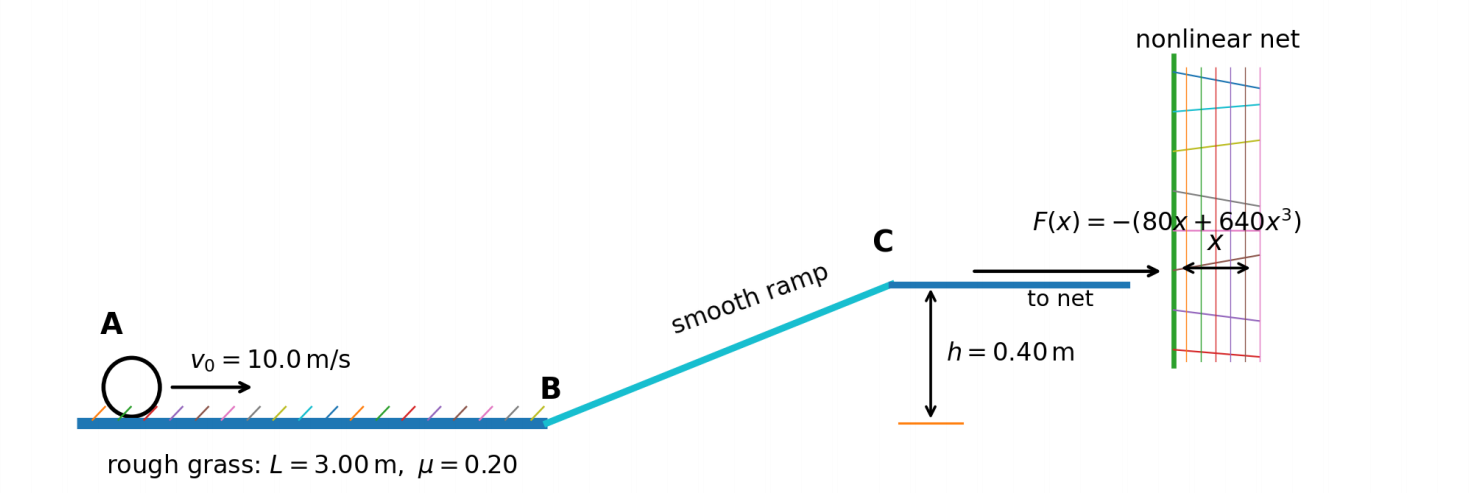
\includegraphics[width=0.92\linewidth]{./fig_6.9/football_net_energy.png}
\end{center}

\begin{enumerate}
 \item 求足球刚离脚时的动能，以及到达 $B$ 点时的动能和速度。
 \item 求足球刚到达球网前，也就是 $C$ 点处的动能和速度。
 \item 推导球网的势能函数 $U_{\mathrm{net}}(x)$，并求足球压入球网的最大深度 $x_{\max}$。判断足球能否在碰到硬质支架前停下。
 \item 若球网把足球完全弹回，足球沿原路返回，经过坡道后再次穿过粗糙草地 $BA$。求足球回到 $A$ 点时的动能和速度。
 \item 结合本题说明，哪些力可以引入势能，哪些力不能引入势能。并判断每一段是否可用机械能守恒。
\end{enumerate}
\end{problemBox}

\section*{详细解法}

\subsection*{一、从 $A$ 到 $B$：动能定理处理粗糙草地}
刚离脚时，足球的动能为
\[
 K_A=\frac{1}{2}mv_0^2=\frac{1}{2}\times 0.50\times (10.0)^2=25.0\,\mathrm{J}.
\]
在粗糙草地上，动摩擦力大小为 $\mu mg$，方向与足球位移方向相反。摩擦力做功为
\[
 W_f=-\mu mgL=-0.20\times 0.50\times 10.0\times 3.00=-3.00\,\mathrm{J}.
\]
由动能定理，
\[
 K_B=K_A+W_f=25.0-3.00=22.0\,\mathrm{J}.
\]
于是
\[
 v_B=\sqrt{\frac{2K_B}{m}}=\sqrt{\frac{2\times 22.0}{0.50}}
=\sqrt{88}\approx 9.38\,\mathrm{m/s}.
\]
这一段不能使用机械能守恒，因为动摩擦力造成机械能耗散。

\subsection*{二、从 $B$ 到 $C$：光滑坡道上的动能与重力势能转化}
坡道光滑，支持力不做功，只有重力做功，因此机械能守恒。足球从高度 $0$ 上升到高度 $h$，重力势能增加
\[
 \Delta U_g=mgh=0.50\times 10.0\times 0.40=2.00\,\mathrm{J}.
\]
所以 $C$ 点处的动能为
\[
 K_C=K_B-mgh=22.0-2.00=20.0\,\mathrm{J}.
\]
对应速度为
\[
 v_C=\sqrt{\frac{2K_C}{m}}=\sqrt{\frac{2\times 20.0}{0.50}}
=\sqrt{80}\approx 8.94\,\mathrm{m/s}.
\]

\subsection*{三、压入球网：由非线性保守力构造势能}
球网回复力只与压入深度 $x$ 有关，且形变过程无能量损失，因此可以把它看成一维保守力。保守力与势能满足
\[
 F(x)=-\frac{\dd U_{\mathrm{net}}}{\dd x}.
\]
由
\[
 F(x)=-(80x+640x^3)
\]
可得
\[
 \frac{\dd U_{\mathrm{net}}}{\dd x}=80x+640x^3.
\]
取 $U_{\mathrm{net}}(0)=0$，积分得到
\[
 U_{\mathrm{net}}(x)=\int_0^x (80\xi+640\xi^3)\,\dd\xi
=40x^2+160x^4.
\]
最大压入深度处，足球瞬时速度为零，$C$ 点动能全部转化为球网势能：
\[
 40x_{\max}^2+160x_{\max}^4=20.0.
\]
令 $y=x_{\max}^2$，得到
\[
 160y^2+40y-20=0,
\]
两边除以 $20$，得
\[
 8y^2+2y-1=0.
\]
解得正根
\[
 y=\frac{-2+\sqrt{2^2+32}}{16}=\frac{1}{4}.
\]
因此
\[
 x_{\max}=\sqrt{\frac14}=0.50\,\mathrm{m}.
\]
由于 $0.50\,\mathrm{m}<0.55\,\mathrm{m}$，足球能在碰到硬质支架前停下。

\subsection*{四、反弹返回：同一段粗糙草地会再次耗散能量}
球网完全弹回且无能量损失，足球离开球网、回到 $C$ 点时动能仍为
\[
 K_C'=20.0\,\mathrm{J}.
\]
从 $C$ 下滑到 $B$，重力势能减少 $mgh=2.00\,\mathrm{J}$，动能增加到
\[
 K_B'=K_C'+mgh=20.0+2.00=22.0\,\mathrm{J}.
\]
足球再从 $B$ 穿过粗糙草地回到 $A$。虽然运动方向改变了，但动摩擦力仍与位移方向相反，所以摩擦力做功仍为
\[
 W_f'=-\mu mgL=-3.00\,\mathrm{J}.
\]
于是
\[
 K_A'=K_B'+W_f'=22.0-3.00=19.0\,\mathrm{J}.
\]
回到 $A$ 点时的速度大小为
\[
 v_A'=\sqrt{\frac{2K_A'}{m}}=\sqrt{\frac{2\times 19.0}{0.50}}
=\sqrt{76}\approx 8.72\,\mathrm{m/s}.
\]
整个往返过程中，粗糙草地被经过两次，机械能总损失为
\[
 2\mu mgL=6.00\,\mathrm{J},
\]
这也正好等于 $25.0\,\mathrm{J}-19.0\,\mathrm{J}$。

\subsection*{五、力的分类与机械能守恒判断}
\begin{center}
\renewcommand{\arraystretch}{1.35}
\begin{tabular}{>{\centering\arraybackslash}p{2.7cm}>{\centering\arraybackslash}p{3.2cm}>{\centering\arraybackslash}p{3.2cm}>{\centering\arraybackslash}p{4.4cm}}
\toprule
阶段 & 主要力 & 是否可引入势能 & 能量处理方式 \\
\midrule
粗糙草地 $AB$ & 动摩擦力 & 不能 & 用动能定理或非保守力做功 \\
光滑坡道 $BC$ & 重力、支持力 & 重力可以 & 机械能守恒，$K+U_g$ 不变 \\
球网压缩 & 非线性回复力 & 可以 & 机械能守恒，$K+U_{\mathrm{net}}$ 不变 \\
返回草地 $BA$ & 动摩擦力 & 不能 & 摩擦力继续做负功 \\
\bottomrule
\end{tabular}
\end{center}

\section*{答案汇总}
\begin{ideaBox}
\begin{enumerate}
 \item $K_A=25.0\,\mathrm{J}$，$K_B=22.0\,\mathrm{J}$，$v_B\approx 9.38\,\mathrm{m/s}$。
 \item $K_C=20.0\,\mathrm{J}$，$v_C\approx 8.94\,\mathrm{m/s}$。
 \item $U_{\mathrm{net}}(x)=40x^2+160x^4$，$x_{\max}=0.50\,\mathrm{m}$。足球能在碰到硬质支架前停下。
 \item $K_A'=19.0\,\mathrm{J}$，$v_A'\approx 8.72\,\mathrm{m/s}$。
 \item 重力和球网回复力可以引入势能；动摩擦力不能引入势能。光滑坡道和无损球网阶段可用机械能守恒，粗糙草地阶段不能用机械能守恒。
\end{enumerate}
\end{ideaBox}

\section*{技巧与知识点}
\begin{tipBox}
\begin{enumerate}
 \item \textbf{非保守力用做功处理。} 粗糙草地上动摩擦力的功为 $W_f=-\mu mgL$。来回各走一次，就损失两次，而不是互相抵消。
 \item \textbf{势能来自保守力，不来自公式记忆。} 普通弹簧有 $U=\frac12kx^2$，是因为 $F=-kx$。本题中 $F=-(80x+640x^3)$，所以必须从 $F=-\dd U/\dd x$ 出发积分。
 \item \textbf{方程降阶技巧。} 看到 $x^2$ 与 $x^4$ 同时出现，可令 $y=x^2$，把四次方程变成二次方程。本题的关键方程就是 $8y^2+2y-1=0$。
 \item \textbf{支持力通常不改变机械能。} 在光滑坡道上，支持力始终垂直于位移，不做功；真正参与能量转化的是重力。
\end{enumerate}
\end{tipBox}

\section*{常见误区}
\begin{warnBox}
\begin{enumerate}
 \item \textbf{误区一：把非线性球网当成普通弹簧。} 如果直接写 $U=\frac12kx^2$，就等于忽略了 $640x^3$ 这一项，题目的主要考点会丢掉。
 \item \textbf{误区二：认为反弹回来可以抵消摩擦损失。} 摩擦力的方向总是与相对运动方向相反，正向通过草地和反向通过草地都做负功。
 \item \textbf{误区三：把能量守恒和机械能守恒混在一起。} 总能量总是守恒，但机械能不一定守恒。机械能减少时，通常转化成内能、声能等形式。
 \item \textbf{误区四：只看初末高度，不看中途耗散。} 本题起点和返回点高度相同，但返回速度变小，原因正是草地两次耗散机械能。
\end{enumerate}
\end{warnBox}

\section*{复习建议}
\begin{tipBox}
第4章动能与势能适合按下面的顺序复习。
\begin{enumerate}
 \item \textbf{先背定义，再背适用条件。} 动能定理适用范围很广；机械能守恒只适用于非保守力不做功或做功为零的情形。复习时把这两句话放在公式前面。
 \item \textbf{建立三类力清单。} 重力、理想弹簧力、只与位置有关且无滞后的回复力，通常可以配势能；动摩擦力、空气阻力、碰撞损失，通常不能配势能。

 \item \textbf{专门练积分求势能。} 遇到 $F(x)$ 不是简单的 $-kx$ 时，先写
 \[
 U(x)-U(0)=-\int_0^x F(\xi)\,\dd\xi.
 \]
 这个式子比死记弹簧势能更可靠。
 \item \textbf{训练时按难度递进。} 第一轮做只含重力势能的题；第二轮加入摩擦力做功；第三轮加入弹性势能；最后再做本题这种非线性势能加分段耗散的综合题。
 \item \textbf{检查答案是否合乎物理直觉。} 经过粗糙草地后速度应变小；压入球网越深，回复力应越大；反弹回到起点时速度应小于初速度。若结果违背这些直觉，优先检查符号和做功方向。
\end{enumerate}
\end{tipBox}

\end{document}
